%--------------------------------------------------------------------------
\chapter{APPLICATIONS AND CONCLUSION}

%--------------------------------------------------------------------------
\begin{lstlisting}[caption={},label={}]
int main(int argc, char *argv[]) {
    if (argc < 3) {
        printf("Enter a problem size and a row!\n");
        return -1;
    }

    common_data commonData;
    createCommonData(&commonData, argc, argv);

    thread_data data;
    createThreadData(&data, &commonData);

    clock_t start = clock();
    writeSolutions(&data, &commonData, 0, commonData.numTops);

    printf("%f seconds elapsed.\n", ((double) (clock() - start)) / CLOCKS_PER_SEC);
    printf("%lu solutions found!\n", data.counter);

    destroyThreadData(&data);
    destroyCommonData(&commonData);

    return 0;
}
\end{lstlisting}

\begin{enumerate}
\item
\addtocounter{enumi}{1}
\end{enumerate}

%--------------------------------------------------------------------------
\begin{lstlisting}[caption={},label={}]
class thread_manager {
public:
    thread_manager(int argc, char *argv[]) : threadData(std::thread::hardware_concurrency()) {
        createCommonData(&commonData, argc, argv);

        for (auto &data: threadData)
            createThreadData(&data, &commonData);
    }

    ~thread_manager() {
        for (auto &data: threadData)
            destroyThreadData(&data);

        destroyCommonData(&commonData);
    }

    long long runThreads() {
        auto numThreads = threadData.size();

        auto doWork = [this, &numThreads](int i, length startTop, length endTop) {
            writeSolutions(&threadData[i], &commonData, startTop, endTop);
            std::lock_guard<std::mutex> lock(mutex);
            numThreads--;
            condition.notify_one();
        };

        length startTop = 0;
        length offset = commonData.numTops / numThreads;
        auto maxThreads = numThreads - 1;
        auto startTime = std::chrono::high_resolution_clock::now();

        for (auto i = 0; i < maxThreads; ++i) {
            std::thread(doWork, i, startTop, startTop + offset).detach();
            startTop += offset;
        }

        doWork(maxThreads, startTop, commonData.numTops);

        std::unique_lock<std::mutex> lock(mutex);
        condition.wait(lock, [&numThreads] { return numThreads == 0; });

        auto stopTime = std::chrono::high_resolution_clock::now();
        auto duration = std::chrono::duration_cast<std::chrono::milliseconds>(stopTime - startTime);

        return duration.count();
    }

    length getNumSolutions() const {
        length numSolutions = 0;

        for (auto &data: threadData)
            numSolutions += data.counter;

        return numSolutions;
    }

private:
    std::vector<thread_data> threadData;
    common_data commonData;
    std::mutex mutex;
    std::condition_variable condition;
};
\end{lstlisting}

\begin{enumerate}
\item
\addtocounter{enumi}{1}
\end{enumerate}

%--------------------------------------------------------------------------
\begin{lstlisting}[caption={},label={}]
int main(int argc, char *argv[]) {
    if (argc < 3) {
        printf("Enter a problem size and a row!\n");
        return -1;
    }

    thread_manager threadManager(argc, argv);
    std::cout << threadManager.runThreads() << " milliseconds elapsed." << std::endl;
    std::cout << threadManager.getNumSolutions() << " solutions found!" << std::endl;

    return 0;
}
\end{lstlisting}

\begin{enumerate}
\item
\addtocounter{enumi}{1}
\end{enumerate}

We conclude this section with a musical example of how self-derivation may be achieved in a $6 \times 144$ matrix by exploring the symmetries of an aggregate realization.

\begin{example}
    \label{ex:stingray}
    Consider the aggregate realization A.
    \begin{equation}
        A = \begin{tikzcd}
            & 0 \arrow[dddr] && 1 \arrow[dddr] & \\
            & 4 \arrow[ddr] && 5 \arrow[ddr] & \\
            & 8 \arrow[dr] && 9 \arrow[dr] & \\
            * \arrow[ur] \arrow[uur] \arrow[uuur] \arrow[dr] \arrow[ddr] \arrow[dddr] && * \arrow[ur] \arrow[uur] \arrow[uuur] \arrow[dr] \arrow[ddr] \arrow[dddr] && * \\
            & 11 \arrow[ur] && 10 \arrow[ur] & \\
            & 7 \arrow[uur] && 6 \arrow[uur] & \\
            & 3 \arrow[uuur] && 2 \arrow[uuur] &
        \end{tikzcd} \enspace.
    \end{equation}
    It is easily seen that $A$ is invariant under the set of operations $\Omega = \{ \T_0, \T_4, \T_8, \T_3\I, \T_7\I, \T_{11}\I \}$. Thus if $\rho \in \Toc(A)$, then also $\Omega_i(\rho) \in \Toc(A)$. It is also easy to see that $\R(\rho) \in \Toc(\R \circ \Omega_i(A))$. Now let $S = \{ 0, 1, 5, 8, 9, 4, 10, 3, 7, 6, 2, 11 \}$, and consider the combination matrix $\mathcal{A} = [\mathcal{A}_1 | \cdots | \mathcal{A}_6]$.
    \begin{equation}
        \mathcal{A} = \left[
        \begin{array}{cc|cc|cc|cc|cc|cc}
            0 & 1 & 5 & 8 & 9 & 4 & 10 & 3 & 7 & 6 & 2 & 11 \\
            4 & 5 & 9 & 0 & 1 & 8 & 2 & 7 & 11 & 10 & 6 & 3 \\
            8 & 9 & 1 & 4 & 5 & 0 & 6 & 11 & 3 & 2 & 10 & 7 \\
            11 & 10 & 6 & 3 & 2 & 7 & 1 & 8 & 4 & 5 & 9 & 0 \\
            7 & 6 & 2 & 11 & 10 & 3 & 9 & 4 & 0 & 1 & 5 & 8 \\
            3 & 2 & 10 & 7 & 6 & 11 & 5 & 0 & 8 & 9 & 1 & 4
        \end{array}
        \right] \enspace.
    \end{equation}
    By construction, every row of $\mathcal{A}$ is an $\Omega$-transform of $S$. Also by construction, every $\mathcal{A}_i$ is an instance of either $A$ or $\R(A)$, seen as a columnar aggregate, and thus $\Omega$-invariant. It follows we can derive a transform of $S$ from every $\mathcal{A}_i$. Since $\T_7(S) \in \Toc(\mathcal{A}_1)$ and $\R\T_0\I(S) \in \Toc(\mathcal{A}_2)$, we get the self-derivation matrix $X$.
    \begin{equation}
        X = \left[
        \begin{array}{cccccccccccc|cccccccccccc}
            &&&&& 11 && 10 &&&&&&& 6 &&&&& 3 &&&& \\
            &&&& 4 && 5 &&&&&&&&&& 9 &&&&&&& 0 \\
            &&& 3 &&&&& 2 &&&&& 10 &&&&&&&& 7 && \\
            && 0 &&&&&&& 1 &&&&&& 5 &&& 8 &&&&& \\
            & 8 &&&&&&&&& 9 && 1 &&&&&&&& 4 &&& \\
            7 &&&&&&&&&&& 6 &&&&&& 2 &&&&& 11 &
        \end{array}
        \right] \enspace.
    \end{equation}
    It is important to point out that, although we could extend the matrix $X$ to a $6 \times 144$ derivation matrix wherein all columns of $\mathcal{A}$ are presented, we could not do so with arbitrary transforms of $S$. Upon inspection, we see that the transforms of $S$ we can derive from $\mathcal{A}_1$ and $\mathcal{A}_5$ are in
    \begin{equation}
        \{ \T_3, \T_7, \T_{11}, \R\T_1, \R\T_5, \R\T_9, \T_0\I, \T_4\I, \T_8\I, \R\T_2\I, \R\T_6\I, \R\T_{10}\I \} \enspace.
    \end{equation}
    For the columns $\mathcal{A}_2, \mathcal{A}_3, \mathcal{A}_4$ and $\mathcal{A}_6$, we can derive transforms of $S$ that are in
    \begin{equation}
        \{ \T_1, \T_5, \T_9, \R\T_3, \R\T_7, \R\T_{11}, \T_2\I, \T_6\I, \T_{10}\I, \R\T_0\I, \R\T_4\I, \R\T_8\I \} \enspace.
    \end{equation}
    Rather than a hinderance, one could take advantage of this fact by exploring contrasting harmonic regions. Fig.~\ref{fig:stingray} shows a musical realization of $X$:
    \begin{figure}[htbp]
        \centering
        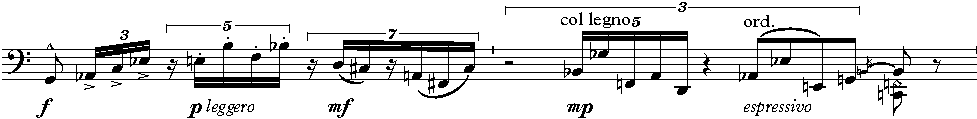
\includegraphics[width=6.5in]{figures/stingray-example.pdf}
        \caption[Self-derivation in Damiani's \emph{Stingray}.]{Self-derivation in Damiani's \emph{Stingray}.}
        \label{fig:stingray}
    \end{figure}
\end{example}

\subsection{Directions for the future}

Vectorize vector addition and subtraction.
